\documentclass[a4paper,11pt]{article}

% Identificação
\newcommand{\pbtitulo}{Pig}
\newcommand{\pbversao}{1.02}

\usepackage{../../sty/tutorial}

%----------------------------------------------------------------------
% Início do Documento
%----------------------------------------------------------------------
\begin{document}
	
	\maketitle % mostrar o título
	\thispagestyle{fancy} % habilitar o cabeçalho/rodapé das páginas
	
%--------------------------------------------------------------------------
% RESUMO DO ARTIGO
%--------------------------------------------------------------------------
\begin{abstract}
	% O primeiro caractere deve vir com \initial{}
	\initial{P}ig\cite{pigoficial} ou "Apache Pig" (aqui chamarei apenas de Pig) é parte do Ecosistema Hadoop criado para ser uma linguagem de script usada para explorar largos datasets. \textit{Pig Latin} é uma extensão do Hadoop, foi desenvolvida pelo Yahoo, para simplificar a programação em alto nível de processamento.
\end{abstract}

%--------------------------------------------------------------------------
% CONTEÚDO DO ARTIGO
%--------------------------------------------------------------------------
\section{Parte inicial}
Pig é uma plataforma ou ferramenta de alto nível que é usada para processar grandes conjuntos de dados. Fornece um alto nível de abstração para processamento no \textit{MapReduce} e uma linguagem de script de alto nível, conhecida como \textit{Pig Latin}, que é usada para desenvolver os códigos de análise de dados.
\begin{figure}[H]
	\centering
	
\includegraphics[width=0.5\textwidth]{imagem/logo}
	\caption{Logo do Apache Pig}
\end{figure}

No início de 2006, Pig foi desenvolvido pelos pesquisadores do Yahoo. Naquela época, a principal ideia para desenvolver uma ferramenta para executar os trabalhos MapReduce em conjuntos de dados extremamente grandes (mesma ideia e mesmo objetivo do Apache Hive). No ano de 2007, mudou-se para Apache Software Foundation (ASF) como um projeto de código aberto. A primeira versão (0.1) veio no ano de 2008.

Componentes do Pig: \vspace{-1em}
\begin{itemize}
	\item \textit{Pig Latin} - Linguagem utilizada para expressar fluxos de dados.
	\item \textit{Pig Engine} - O motor no topo do hadoop
\end{itemize}
	
Para processar os dados armazenados no HDFS, escrevemos \textit{scripts} usando a \textit{Pig Latin Language}. Internamente o \textit{Pig Engine} (motor do Pig) converte todos esses \textit{scripts} em um mapa específico e tarefa de redução. Mas estes não ficam visíveis para os programadores por fornecerem um alto nível de abstração. Pig Latin e Pig Engine são os dois principais componentes da ferramenta Apache Pig. O resultado do Pig sempre armazenado no HDFS.	

Aplicações do Pig: \vspace{-1em}
\begin{itemize}
	\item Para explorar grandes conjuntos de dados, o Pig Scripting é usado.
	\item Fornecer suporte em grandes conjuntos de dados para consultas Ad-hoc.
    \item Na prototipagem de algoritmos de processamento de grandes conjuntos de dados.
    \item Processar as cargas de dados sensíveis ao tempo.
    \item coletar grandes quantidades de conjuntos de dados na forma de logs de pesquisa e rastreamentos da web.
    \item Em respostas analíticas quando é necessário usar amostragem.
\end{itemize}

Tipos de modelos de dados no Pig: \vspace{-1em}
\begin{itemize}
	\item \textit{Atom}: Valor de dados atômicos que é usado para armazenar como uma string. O principal uso deste modelo é poder ser usado como um número e também como uma string.
	\item \textit{Tuple}: Conjunto ordenado dos campos.
	\item \textit{Bag}: Coleção de tuplas.
	\item \textit{Map}: Conjunto de pares chave/valor.
\end{itemize}

\section{Hadoop no Docker}
O modo mais simples de se conseguir trabalhar com o Hadoop é utilizando o Docker, para baixar a imagem do Hadoop: \\
\codigo{\$ docker pull suhothayan/hadoop-spark-pig-hive:2.9.2}

Nessa imagem temos outros produtos do Ecossistema Hadoop: Spark, Pig e Hive. Para criar e executar a primeira vez o contêiner (a pasta que este comando for executado será associada a uma pasta interna chamada \textbf{/home/tsthadoop}): \\
\codigo{\$ docker run -it -d --name meu-hadoop -v \$(pwd):/home/tsthadoop \\ suhothayan/hadoop-spark-pig-hive:2.9.2}

Uma vez interrompido o contêiner: \\
\codigo{\$ docker stop meu-hadoop}

Podemos executá-lo novamente com os seguintes comandos: \\
\codigo{\$ docker start meu-hadoop \\
\$ docker exec -it meu-hadoop /etc/bootstrap.sh bash}

\subsection{Erro de Permissão}
Na primeira vez que entramos é dado um erro na execução do script "bootstrap.sh" de permissão negada para executar o script "spark-env.sh", vamos corrigir isso com o comando: \\
\codigo{\# chmod 777 /usr/local/spark/conf/spark-env.sh}

Vamos sair do bash: \\
\codigo{\# exit}

Podemos executá-lo novamente: \\
\codigo{\$ docker exec -it meu-hadoop /etc/bootstrap.sh bash}

E o erro desapareceu.


E podemos verificar a versão do Hadoop e Pig que estão instalados: \\
\codigo{\$ hadoop version \\
\$ pig --version}

O endereço da pasta do Pig: \\
\codigo{\$ cd /usr/local/pig}

\subsection{Modos de Execução}
Pig pode ser executado de duas maneiras diferentes:
\begin{figure}[H]
	\centering
	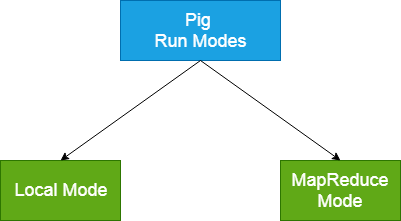
\includegraphics[width=0.5\textwidth]{imagem/modos}
	\caption{Modos de Execução}
\end{figure}

\textbf{Modo local} - executado em uma única JVM e é usado para experimentação e prototipagem de desenvolvimento. Desta maneira os arquivos são instalados e executados usando localhost. O modo local funciona em um sistema de arquivos local. Os dados de entrada e saída armazenados no sistema de arquivos local. \\
\codigo{\$ pig -x local}

\textbf{Modo MapReduce} - também é conhecido como modo Hadoop. É o modo padrão. Neste Pig renderiza Pig Latin em trabalhos MapReduce e os executa no cluster. Pode ser executado em uma instalação do Hadoop semi-distribuída ou totalmente distribuída. Aqui, os dados de entrada e saída estão presentes no HDFS. \\
\codigo{\$ pig}

Ou então \\
\codigo{\$ pig -x mapreduce}

Para executar um Script em Pig temos as seguintes maneiras: \vspace{-1em}
\begin{itemize}
	\item \textbf{Modo Interativo} - Neste modo, o Pig é executado no shell do Grunt. Para invocar o shell Grunt, execute o comando pig. Uma vez que o modo Grunt é executado, podemos fornecer instruções e comandos Pig Latin interativamente na linha de comando.
	\item \textbf{Modo em Lote} - Neste modo, podemos executar um arquivo de script com extensão .pig. Esses arquivos contêm comandos do Pig Latin.
	\item \textbf{Modo Embutido} - Neste modo, podemos definir nossas próprias funções. Essas funções podem ser chamadas como UDF (Funções Definidas pelo Usuário). Aqui, usamos linguagens de programação como Java e Python.
\end{itemize}

\subsection{Pig Latin}
Sabemos que a \textit{Pig Latin} é uma linguagem de fluxo de dados usada para analisar os dados no Hadoop. É uma linguagem textual que abstrai a programação do idioma Java MapReduce em uma notação.

Tipos de Dados: \vspace{-1em}
\begin{itemize}
	\item \textbf{int} - Inteiro de 32-bit. Exemplo: 2
	\item \textbf{long} - Inteiro de 64-bit. Exemplo: 2L ou 2l
	\item \textbf{float} - Numérico flutuante de 32-bit. Exemplo: 2.5F, 2.5f, 2.5e2f ou 2.5.E2F
	\item \textbf{double} - Numérico flutuante de 64-bit. Exemplo: 2.5, 2.5, 2.5e2 ou 2.5.E2
	\item \textbf{chararray} - Array de caracteres em formato Unicode UTF-8. Exemplo: "Fernando"
	\item \textbf{bytearray} - Array de bytes.
	\item \textbf{boolean} - Tipo lógico que pode conter os valores true/false.
	\item \textbf{datetime} - Tipo data/hora no formato padrão. Exemplo: 2022-03-02T12:54:00.000+00:00
	\item \textbf{biginteger} - Tipo Java BigInteger para inteiros gigantes.
	\item \textbf{bigdecimal} - Tipo Java BigDecimal para numéricos flutuantes gigantes.
\end{itemize}

Como dito anteriormente, temos ainda os tipos complexos: \vspace{-1em}
\begin{itemize}
	\item \textbf{tuple} - Um conjunto ordenado de campos. Exemplo: (15,12)
	\item \textbf{bag} - Uma coleção de tuplas. Exemplo: \{(15,12), (15,22)\}
	\item \textbf{map} - Um conjunto de chaves e valores. Exemplo: [chv1\#valor]
\end{itemize}

\section{Pig com o HDFS}
Antes de fazermos qualquer coisa no Pig precisamos ativar o JobHistory (que por padrão está inativo):
\codigo{\# ./usr/local/hadoop-2.9.2/sbin/mr-jobhistory-daemon.sh --config /usr/local/hadoop/etc start historyserver}

Para praticarmos um pouco temos um arquivo CSV (que foi disponibilizado na pasta dados em \url{https://github.com/fernandoans/publicacoes/tree/master/Apostilas/Pig/dados}) chamado SalesJan2009.csv que representa um conjunto de vendas. Nosso primeiro trabalho será colocá-lo a disposição do HDFS.

Colocar o arquivo na pasta associativa do contêiner do Docker (lembramos que existe uma pasta interna que faz as associações quando o contêiner é ativo). Em seguida dentro do contêiner acesse a pasta associativa: \\
\codigo{\# cd /home/tsthadoop}

Se verificarmos o conteúdo da pasta: \\
\codigo{\# ls}

O arquivo CSV indicado deve estar nela. Para adicioná-lo ao HDFS: \\
\codigo{\# hadoop fs -put SalesJan2009.csv}

E verificamos se o arquivo foi adicionado ao HDFS: \\
\codigo{\# hadoop dfs -ls} 

Que deve mostrar o seguinte resultado:
\begin{figure}[H]
	\centering
	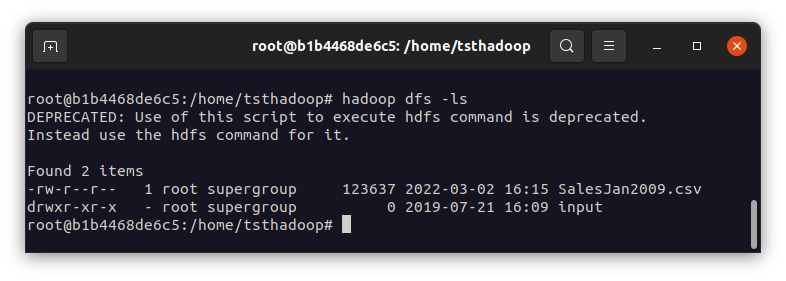
\includegraphics[width=0.8\textwidth]{imagem/listagem}
	\caption{Arquivo no HDFS}
\end{figure}

Ativamos o Pig em modo MapReduce: \\
\codigo{\# pig} 

No Grunt que é comando prompt do Pig. Executamos o seguinte comando para ler os dados: \\
\codigo{grunt> salesTable = LOAD 'SalesJan2009.csv' USING PigStorage(',') AS \\ (Transaction\_date:chararray,Product:chararray,Price:chararray, \\
Payment\_Type:chararray,Name:chararray,City:chararray,State:chararray, \\ Country:chararray,Account\_Created:chararray,Last\_Login:chararray, \\
Latitude:chararray,Longitude:chararray);}

Criar um grupo por País: \\
\codigo{grunt> GroupByCountry = GROUP salesTable BY Country;}

Para cada tupla em ‘GroupByCountry’, gerar uma string resultante do formulário-> Nome do País: Nº de produtos vendidos: \\
\codigo{grunt> CountByCountry = FOREACH GroupByCountry \\
GENERATE CONCAT((chararray)\$0,CONCAT(':',(chararray)COUNT(\$1)));}

Armazenar o resultado em um Fluxo de Dados chamado "pig\_saida\_vendas": \\
\codigo{grunt> STORE CountByCountry INTO 'pig\_saida\_vendas' USING PigStorage('$\setminus$t');}

E quando esse último comando for colocado a mágica começa, e um MapReduce é iniciado realizando todo o trabalho, pensando no Hadoop isso evita de termos de pensar em criar Scripts para realizar o Map/Reduce.

Saímos do Pig com CTRL+C e damos o seguinte comando para vermos o resultado: \\
\codigo{\# hdfs dfs -cat pig\_saida\_vendas/part-r-00000}

Outra forma de visualizarmos os resultados é através do navegador acessando o HDFS em \url{http://localhost:50070}, na página acessar no menu superior as opções: Utilities | Browse the file system. Na página navegar para o diretório: /user/root e temos o seguinte resultado:
\begin{figure}[H]
	\centering
	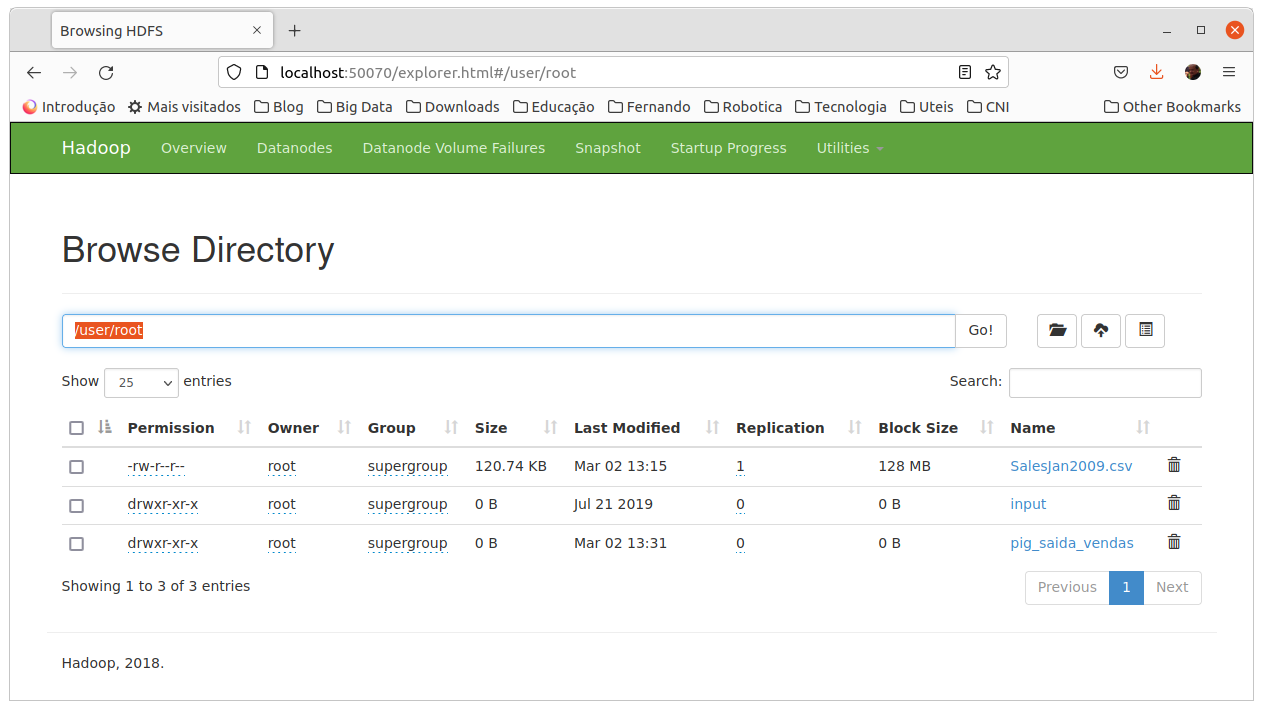
\includegraphics[width=0.8\textwidth]{imagem/hdfsbrowser}
	\caption{Arquivo no HDFS no Navegador}
\end{figure}

Clicar em pig\_saida\_vendas e temos o arquivo que foi gerado. Percebeu que podemos fazer muita coisa nessa página como adicionar ou remover arquivos e pastas ou navegar por todas as pastas existentes no HDFS. Aconselho que explore bem essa página e suas funcionalidades.

\subsection{Pig Script}
Outra forma de fazermos o mesmo trabalho seria a criação de um Script, para isso, digite o seguinte comando: \\
\codigo{\# vim pigvenda.pig}

Digite "i" (para entrar em modo de inserção) e insira a seguinte codificação:
\begin{lstlisting}[]
salesTable = LOAD 'SalesJan2009.csv' USING PigStorage(',') AS (Transaction_date:chararray, Product:chararray, Price:chararray, Payment_Type:chararray, Name:chararray, City:chararray, State:chararray, Country:chararray, Account_Created:chararray, Last_Login:chararray, Latitude:chararray, Longitude:chararray);
GroupByCountry = GROUP salesTable BY Country;
CountByCountry = FOREACH GroupByCountry GENERATE CONCAT((chararray)$0,CONCAT(':',(chararray)COUNT($1)));
STORE CountByCountry INTO 'pig_saida2_vendas' USING PigStorage('\t');
\end{lstlisting}

Para salvar pressionar ESC (para sair do modo de inserção) e ":wq" para salvar e sair. Para executar: \\
\codigo{\# pig pigvenda.pig}

Fantástico isso não, as mesmas ações serão executadas só que agora através de um Script que pode ser guardado e executado para futuras modificações no arquivo. Verifique que novamente foi gerado o arquivo de saída (agora com outro nome): \\
\codigo{\# hdfs dfs -cat pig\_saida2\_vendas/part-r-00000}

Como diria Jack vamos por partes. Então em cada subseção abaixo vamos nos concentrar somente no operador em questão para entender o que cada um deles realiza, e assim termos uma ideia do que podemos obter com Pig.

\subsection{Operador Load}
Utilizado para ler dados do sistema de arquivos HDFS, sua sintaxe é: \\
\codigo{LOAD 'arquivo' [USING tipo] [AS estrutura];}

Por exemplo, vamos supor que temos o seguinte arquivo (criar com o nome notas.txt e em seguida adicioná-lo ao HDFS):
\begin{lstlisting}[]
Joana,5.0,6.0,7
Carlos,7.0,3.0,8
Marla,6.5,4.2,7
\end{lstlisting}

Contendo o nome, notas e total de faltas dos alunos em uma determinada matéria. Desejamos ler esses dados. \\
\codigo{grunt> tabnotas = LOAD 'notas.txt' USING PigStorage(',') AS (nome:chararray, \\
nota1:double, nota2:double, faltas:int);}

Vamos executar esse comando: \\
\codigo{grunt> DUMP tabnotas;}

E verificar o resultado: \\
\codigo{grunt> DESCRIBE tabnotas;}

Obviamente é bem mais interessante utilizar esse operador em combinação com outros.

\subsection{Operador Store}
Utilizado para armazenar ou salvar resultados no sistema de arquivos HDFS, sua sintaxe é: \\
\codigo{STORE arquivo INTO 'diretorio' [USING funcao];}

Por exemplo, vamos supor o arquivo "notas.txt" criado anteriormente. Lemos seus dados. \\
\codigo{grunt> tabnotas = LOAD 'notas.txt' USING PigStorage(',') AS (nome:chararray, \\
nota1:double, nota2:double, faltas:int);}

Vamos executar esse comando: \\
\codigo{grunt> DUMP tabnotas;}

E podemos armazenar o resultado no HDFS: \\
\codigo{grunt> STORE tabnotas INTO 'saidaNotas' USING PigStorage('*'); \\
grunt> CAT saidaNotas;}

E teremos com resultado do processo:
\begin{lstlisting}[]
nome***
Joana*5.0*6.0*7
Carlos*7.0*3.0*8
Marla*6.5*4.2*7
\end{lstlisting}

Ficou separado por '*' pois foi esse caractere que definimos na função "PigStore(char)".

\subsection{Operador Cross}
Operador para facilitar a computação para um produto de duas ou mais relações. Isso facilita enormemente o processamento. Para exemplificarmos seu uso precisamos de dois arquivos, "matriz1.txt" com o seguinte conteúdo:
\begin{lstlisting}[]
1,2
3,4
\end{lstlisting}

E "matriz2.txt" com o seguinte conteúdo:
\begin{lstlisting}[]
5,6,7
8,9,10
\end{lstlisting}

Criar ambos arquivos e adicioná-los ao HDFS. Agora no Pig precisamos ler ambos: \\
\codigo{grunt> arq1 = LOAD 'matriz1.txt' USING PigStorage(',') AS (a1:int,a2:int); \\
grunt> DUMP arq1; \\
grunt> arq2 = LOAD 'matriz2.txt' USING PigStorage(',') AS (b1:int,b2:int,b3:int); \\
grunt> DUMP arq2;}

E agora podemos realizar o relacionamento cruzado entre eles: \\
\codigo{grunt> resultado = CROSS arq1,arq2; \\
grunt> DUMP resultado;}

E teremos com resultado do processo:
\begin{lstlisting}[]
(1,2,5,6,7)
(1,2,8,9,10)
(3,4,5,6,7)
(3,4,8,9,10)
\end{lstlisting}

\subsection{Operador Distinct}
Usado para remover tuplas duplicadas nas relações. Para realizar esse procedimento Pig ordena os dados e elimina os duplicados. Vamos criar o arquivo "dados.txt" com o seguinte conteúdo:
\begin{lstlisting}[]
1,2,3
4,5,6
1,2,3
7,8,9
4,5,6
\end{lstlisting}

Adicioná-lo ao HDFS. Agora no Pig vamos ler o arquivo: \\
\codigo{grunt> arq = LOAD 'dados.txt' USING PigStorage(',') AS (a1:int,a2:int,a3:int); \\
grunt> DUMP arq;}

E aplicamos o comando \textit{distinct}: \\
\codigo{grunt> resultado = DISTINCT arq; \\
grunt> DUMP resultado;}

E teremos com resultado do processo:
\begin{lstlisting}[]
(1,2,3)
(4,5,6)
(7,8,9)
\end{lstlisting}

\subsection{Operador Filter}
Utilizado para remover tuplas da relação que não condizem a um determinado critério, se está tentando associar ao SQL, este operador seria o WHERE. Vamos criar o arquivo "dados.txt" com o seguinte conteúdo:
\begin{lstlisting}[]
1,8
2,8
2,3
8,9
5,8
\end{lstlisting}

Adicioná-lo ao HDFS. Agora no Pig vamos ler o arquivo: \\
\codigo{grunt> arq = LOAD 'dados.txt' USING PigStorage(',') AS (a1:int,a2:int); \\
grunt> DUMP arq;}

E aplicamos o comando \textit{distinct}: \\
\codigo{grunt> resultado = FILTER arq BY a2==8; \\
grunt> DUMP resultado;}

E teremos com resultado do processo:
\begin{lstlisting}[]
(1,8)
(2,8)
(5,8)
\end{lstlisting}

\subsection{Operador ForEach}
Realiza uma interação com cada um dos elementos arrumando-os no formato que desejamos. Vamos criar o arquivo "dados.txt" com o seguinte conteúdo:
\begin{lstlisting}[]
1,2,3
4,5,6
7,8,9
\end{lstlisting}

Adicioná-lo ao HDFS. Agora no Pig vamos ler o arquivo: \\
\codigo{grunt> arq = LOAD 'dados.txt' USING PigStorage(',') AS (a1:int,a2:int,a3:int); \\
grunt> DUMP arq;}

E aplicamos o comando \textit{foreach}: \\
\codigo{grunt> resultado = FOREACH arq GENERATE CONCAT('a:', (chararray)a1), \\
CONCAT('b:', (chararray)a2), CONCAT('c:', (chararray)a3); \\
grunt> DUMP resultado;}

E teremos com resultado do processo:
\begin{lstlisting}[]
(a:1,b:2,c:3)
(a:4,b:5,c:6)
(a:7,b:8,c:9)
\end{lstlisting}

\subsection{Operador Group}
Agrupar um ou mais relacionamento entre os campos, se estiver comparando com o SQL acabou de encontrar o operador GROUP BY, porém aqui temos algo mais especializado. Vamos criar o arquivo "familia.txt" com o seguinte conteúdo:
\begin{lstlisting}[]
Fernando,Anselmo
Jessica,Rabbit
Robin,Batman
Hugo,Anselmo
Roger,Rabbit
Fox,Rabbit
Bruce,Batman
\end{lstlisting}

Adicioná-lo ao HDFS. Agora no Pig vamos ler o arquivo: \\
\codigo{grunt> arq = LOAD 'familia.txt' USING PigStorage(',') AS (n1:chararray, n2:chararray); \\
grunt> DUMP arq;}

E aplicamos o comando \textit{group}: \\
\codigo{grunt> resultado = group arq by n2; \\
grunt> DUMP resultado;}

E teremos com resultado do processo:
\begin{lstlisting}[]
( Batman,{(Bruce,Batman),(Robin,Batman)})
( Rabbit,{(Fox,Rabbit),(Roger,Rabbit),(Jessica,Rabbit)})
( Anselmo,{(Hugo,Anselmo),(Fernando,Anselmo)})
\end{lstlisting}

\subsection{Operador Limit}
Limitar a quantidade das tuplas mostradas, se estiver comparando com o SQL este é o LIMIT (de alguns bancos, pois em outros é TOP), vamos nos aproveitar do arquivo carregado no comando anterior, que ao dar um comando: \\
\codigo{grunt> DUMP arq;}

Temos como saída:
\begin{lstlisting}[]
(Fernando,Anselmo)
(Jessica,Rabbit)
(Robin,Batman)
(Hugo,Anselmo)
(Roger,Rabbit)
(Fox,Rabbit)
(Bruce,Batman)
\end{lstlisting}

E aplicamos o comando \textit{limit}: \\
\codigo{grunt> resultado = LIMIT arq 3; \\
grunt> DUMP resultado;}

Temos como saída:
\begin{lstlisting}[]
(Fernando,Anselmo)
(Jessica,Rabbit)
(Robin,Batman)
\end{lstlisting}

\subsection{Operador Order}
Ordenar as saídas das tuplas mostradas, se estiver comparando com o SQL este é o ORDER BY, vamos nos aproveitar do arquivo carregado no comando GROUP e ordenar sua saída com o comando \textit{order}: \\
\codigo{grunt> resultado = ORDER arq BY n1 ASC; \\
grunt> DUMP resultado;}

Os campos podem ser ordenados de modo descendente (DESC) ou ascendente (ASC). Temos como saída:
\begin{lstlisting}[]
(Fernando,Anselmo)
(Jessica,Rabbit)
(Robin,Batman)
\end{lstlisting}

\subsection{Operador Split}
Cria uma nova saída através de uma condição determinada, porém TODAS as condições de campo devem ser abrangidas, por exemplo: um arquivo que contém 2 gêneros M e F, deve ter uma condição para cada um dos gêneros. Nosso arquivo possui 3 famílias, assim:\\
\codigo{grunt> SPLIT arq INTO famBatman IF EqualsIgnoreCase(n2,'Batman'), \\
famRabbit IF EqualsIgnoreCase(n2,'Rabbit'), \\
famAnselmo IF EqualsIgnoreCase(n2,'Anselmo');}

E podemos aplicar o : \\
\codigo{grunt> DUMP famBatman;}

E temos como saída a família "Batman":
\begin{lstlisting}[]
(Robin,Batman)
(Bruce,Batman)
\end{lstlisting}

\subsection{Operador Union}
Se entendeu o comando Split o Union será extremamente fácil de demonstrar, pois faz exatamente o contrário, vamos juntar as famílias Batman e Rabbit em um único resultado: \\
\codigo{grunt> resultado = UNION famBatman,famRabbit;}

E temos como saída as famílias unidas:
\begin{lstlisting}[]
(Jessica,Rabbit)
(Roger,Rabbit)
(Fox,Rabbit)
(Robin,Batman)
(Bruce,Batman)
\end{lstlisting}

\section{Diversas Atividades}
Esses são alguns problemas que podemos resolver utilizando roteiros do Pig.

\textbf{Problema 1}: Com base no seguinte arquivo denominado \textit{notas.csv}:
\begin{lstlisting}[]
Nome,Nota1,Nota2
Ana,85,92
Pedro,78,90
Mariana,93,88
Luiz,89,76
Rafael,88,95
\end{lstlisting}

Trazer somente  aluna com o nome "Mariana".
\begin{lstlisting}[]
alunos = LOAD 'notas.csv' USING PigStorage(',') AS (Nome:chararray,Nota1:int,Nota2:int);
resultado = FILTER alunos BY Nome=='Mariana';
DUMP resultado;
\end{lstlisting}

\textbf{Problema 2}: Com base no seguinte arquivo denominado \textit{vendedores.csv}:
\begin{lstlisting}[]
id,email,gender,cidade,name
1,raronsohn0@qq.com,Female,Mojo,Reeta Aronsohn
2,jbyles1@delicious.com,Male,Eusébio,Jonathon Byles
3,jbeyne2@icio.us,Male,Stockholm,Jone Beyne
4,ngeroldini3@senate.gov,Female,Yambol,Nyssa Geroldini
\end{lstlisting}

Obter a lista dos vendedores agrupados por Cidade e Gênero, contando os registros e concatenando nomes e emails de cada grupo.
\begin{lstlisting}[]
data = LOAD 'vendedores.csv' USING PigStorage(',') AS (id:int, email:chararray, gender:chararray, cidade:chararray, name:chararray);
grouped_data = GROUP data BY (cidade, gender);
result = FOREACH grouped_data GENERATE
    group.cidade AS cidade,
    group.gender AS gender,
    COUNT(data) AS record_count,
    data.name AS names,
    data.email AS emails;
STORE result INTO 'dados';
\end{lstlisting}

\textbf{Problema 3}: Com base no seguinte arquivo denominado \textit{populacao.csv}:
\begin{lstlisting}[]
Pais,Qtde,Sexo
Portugal,1111129,Feminino
Eslováquia,5904332,Feminino
Itália,8505041,Feminino
Finlândia,3259521,Feminino
Espanha,6814912,Masculino
Eslováquia,4729838,Masculino
França,7780761,Feminino
Espanha,4830073,Masculino
Espanha,472902,Masculino
Portugal,8320889,Masculino
França,5697275,Masculino
\end{lstlisting}

Encontrar a quantidade de pessoas na Espanha.
\begin{lstlisting}[]
base = LOAD 'base_europa.csv' USING PigStorage(',') AS (pais:chararray, qtde:int, sexo:chararray);
resultado = FILTER base by pais=='Espanha';
STORE resultado INTO 'dadEspanha' USING PigStorage('\t');
\end{lstlisting}

\textbf{Problema 4}: Com base no seguinte arquivo denominado \textit{clientes.csv}:
\begin{lstlisting}[]
Id,Genre,Age,Score
0001,Male,19,39
0002,Male,51,81
0003,Female,20,6
0004,Female,23,77
0005,Female,51,40
0006,Female,22,76
0007,Female,55,6
0008,Female,23,94
0009,Male,64,3
0010,Female,30,72
\end{lstlisting}

Encontrar quem entre os clientes possuem um resultado maior que 50 unidades.
\begin{lstlisting}[]
mallCustomers = LOAD 'clientes.csv' USING PigStorage(',') AS (Id:chararray, Genre:chararray, Age:int, Score:int);
filtroRenda = FILTER mallCustomers BY Score >= 50;
groupRenda = GROUP filtroRenda BY Genre;
somarRenda = FOREACH groupRenda GENERATE group AS Genre;
ordenado = ORDER somarRenda BY $1 DESC;
STORE ordenado INTO 'dados' USING PigStorage('\t');
\end{lstlisting}

Problema 5:  Com base no seguinte arquivo denominado \textit{pessoas.csv}:
\begin{lstlisting}[]
Nome,Idade,Cidade
João,25,São Paulo
Maria,30,Rio de Janeiro
Carlos,22,Belo Horizonte
Ana,28,Porto Alegre
Pedro,35,Brasília
Mariana,27,Salvador
Rafael,32,Curitiba
Juliana,29,Recife
\end{lstlisting}

\begin{lstlisting}[]
listTable = LOAD 'pessoas.csv' USING PigStorage(',') AS(Nome:chararray,Idade:int,Cidade:chararray);
GroupByCity = GROUP listTable BY Cidade;
CountByCity = FOREACH GroupByCity GENERATE CONCAT((chararray)$0,CONCAT(':',(chararray)COUNT($1)));
STORE CountByCity INTO 'dados' USING PigStorage('\t');
\end{lstlisting}

\section{Resumão Geral}
Mas afinal de contas qual a vantagem do Pig, pois tudo o que fazemos com ele poderíamos realizar com um SQL no Hive (por exemplo), isso é uma verdade. Porém devemos olhar para o Pig como uma alternativa \textit{Script} que podemos agendar, executar a qualquer momento de um modo simples e prático, basta apenas nos acostumarmos com a sintaxe deste. 

Por exemplo, o seguinte SQL que localiza as vendas superiores a 2.000,00 na cidade do Texas, comparativamente em um Script Pig é escrito do seguinte modo:
\begin{figure}[H]
	\centering
	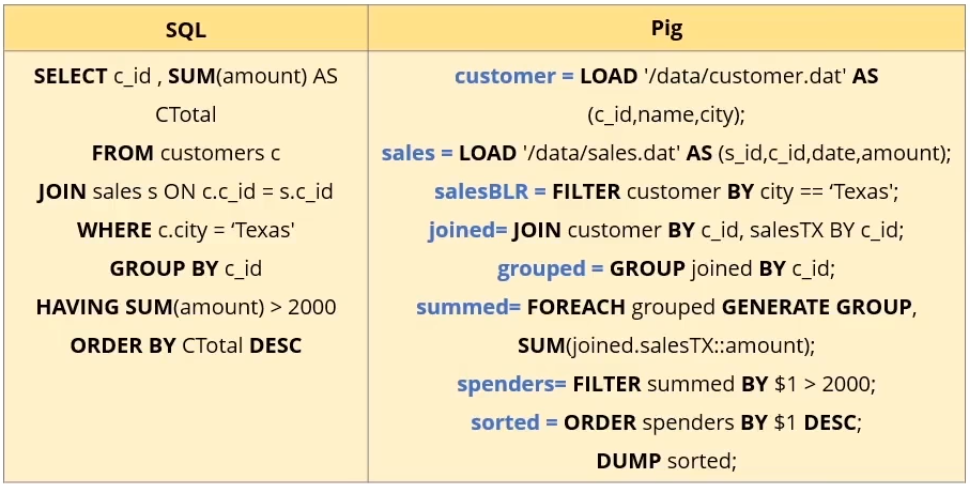
\includegraphics[width=0.8\textwidth]{imagem/vendas}
	\caption{Comparando SQL e Pig Latin}
\end{figure}

Mais fontes de informação podem ser obtidas em diversos sites que apresenta tutoriais completos sobre o Apache Pig como a Tutorials Point\cite{tutorialspoint}.

\section{Conclusão}
Pig é uma plataforma de fluxo de dados de alto nível para executar programas MapReduce do Hadoop. A linguagem usada é a \textit{Pig Latin}. Os scripts Pig são convertidos internamente em tarefas Map Reduce e executados em dados armazenados no HDFS. Além disso, Pig também pode executar seu trabalho no Apache Tez ou no Apache Spark.

Pig pode lidar com qualquer tipo de dados, ou seja, estruturados, semiestruturados ou não estruturados e armazena os resultados correspondentes no Hadoop Data File System. Todas as tarefas que podem ser realizadas usando o PIG também podem ser realizadas usando o java usado no MapReduce. 

Pig consome menos linha de código para realizar qualquer operação. Seu código é flexível o suficiente para ser reutilizado novamente. Fornece um conceito útil de tipos de dados aninhados, como \textit{tuple}, \textit{bag} e \textit{map}.

Sou um entusiasta do mundo \textbf{Open Source} e novas tecnologias. Qual a diferença entre Livre e Open Source? \underline{Livre} significa que esta apostila é gratuita e pode ser compartilhada a vontade. \underline{Open Source} além de livre todos os arquivos que permitem a geração desta (chamados de arquivos fontes) devem ser disponibilizados para que qualquer pessoa possa modificar ao seu prazer, gerar novas, complementar ou fazer o que quiser. Os fontes da apostila (que foi produzida com o LaTex) está disponibilizado no GitHub \cite{github}. Veja ainda outros artigos que publico sobre tecnologia através do meu Blog Oficial \cite{fernandoanselmo}.

%--------------------------------------------------------------------------
% REFERÊNCIAS
%--------------------------------------------------------------------------
\begin{thebibliography}{4}
	\bibitem{pigoficial} 
	Página do Apache Pig \\
	\url{https://pig.apache.org/}

	\bibitem{tutorialspoint} 
	Tutorials Point sobre Pig \\
	\url{https://www.tutorialspoint.com/apache_pig/index.htm}
	
		\bibitem{fernandoanselmo} 
	Fernando Anselmo - Blog Oficial de Tecnologia \\
	\url{http://www.fernandoanselmo.blogspot.com.br/}
	
	\bibitem{publicacao} 
	Encontre essa e outras publicações em \\
	\url{https://cetrex.academia.edu/FernandoAnselmo}
	
	\bibitem{github} 
	Repositório para os fontes da apostila \\
	\url{https://github.com/fernandoans/publicacoes}
\end{thebibliography}

\end{document}